\section{Preprocesamiento de datos}

    Con el objetivo de garantizar la homogeneidad de los corpus empleados y mitigar posibles sesgos derivados de las variaciones en los entornos de grabación (tales como diferencias en la microfonía o ruido de fondo), todas las señales acústicas crudas son sometidas a un pipeline de acondicionamiento estandarizado antes de la fase de extracción de características.

    \subsection{Preprocesamiento de las señales acústicas}

        El flujo de preprocesamiento digital de la señal consta de las siguientes etapas secuenciales:

        \begin{itemize}
            \item \textbf{Conversión de formato y remuestreo:} En primer lugar, aquellas muestras grabadas en formato estereofónico se convierten a monofónico promediando sus canales, reduciendo así la dimensionalidad espacial. Seguidamente, todas las señales se remuestrean a una frecuencia estándar de 16 kHz. Esta frecuencia es el estándar de facto en el modelado acústico moderno, coincidiendo con la frecuencia nativa de entrada de arquitecturas de vanguardia como Wav2Vec 2.0 \cite{baevski2020}, ya que preserva el espectro de frecuencias vocales relevantes minimizando la carga computacional.
            
            \item \textbf{Reducción de ruido (Denoising):} Para eliminar el ruido estacionario de fondo, se aplica un algoritmo de puerta de ruido espectral (\textit{Spectral Gating}) en el dominio espectro-temporal haciendo uso de la librería de Python \textit{noisereduce} \cite{sainburg2024}. Este proceso estima el perfil de ruido a partir de los estadísticos de los canales de frecuencia (calculados desde una muestra de ruido de fondo) y aplica una máscara para atenuarlo. Esto permite mejorar la Relación Señal-Ruido (SNR) preservando la señal de voz sin introducir distorsiones ni artefactos en los formantes fonéticos del paciente.
                
            \item \textbf{Recorte de silencios no fonéticos (\textit{Trimming}):} Finalmente, se eliminan los segmentos de silencio absoluto o ruido ambiente residual presentes al inicio y al final de cada grabación mediante la librería \textit{librosa} \cite{mcfee2015}. Este recorte se realiza identificando los tramos cuya amplitud RMS (\textit{Root Mean Square}) cae por debajo de un umbral de 20 dB respecto al pico máximo de la señal, asegurando que los modelos solo procesen actividad vocal útil.
        \end{itemize}

    \subsection{Extracción de características manuales para Machine Learning Tradicional}
            A partir del preprocesamiento de la señal, se procedió a la extracción de un conjunto de características acústicas diseñadas para capturar las alteraciones neuromotoras del habla. Estas métricas se dividen en cuatro dominios clínicos fundamentales: perturbación de frecuencia, perturbación de amplitud, medidas de ruido y medidas de temblor vocal. La \autoref{tab:caracteristicas_acusticas} detalla la formulación y utilidad de cada una de ellas.
            \\

            \small
            \begin{longtable}[c]{@{} l >{\raggedright\arraybackslash}p{7.8cm} l @{}}
                \toprule
                \textbf{Métrica} & \textbf{Definición clínica / matemática} & \textbf{Ref.} \\
                \midrule
                \endfirsthead

                \multicolumn{3}{c}{\small\textit{(Continuación de la \autoref{tab:caracteristicas_acusticas})}} \\[0.3em]
                \toprule
                \textbf{Métrica} & \textbf{Definición clínica / matemática} & \textbf{Ref.} \\
                \midrule
                \endhead

                \bottomrule
                \endlastfoot

                \multicolumn{3}{@{}l}{\textbf{Medidas de Perturbación de Frecuencia (\textit{Jitter})}} \\
                \midrule
                JITA   & \textit{Absolute Jitter}: Variación absoluta promedio ciclo a ciclo del periodo fundamental. & \cite{praat2018} \\
                rJitter & \textit{Relative Jitter}: Variación relativa promedio del periodo fundamental (en \%). & \cite{praat2018} \\
                RAP    & \textit{Relative Average Perturbation}: Perturbación relativa promediada sobre ventanas de 3 ciclos. & \cite{praat2018} \\
                rPPQ   & \textit{Pitch Period Perturbation Quotient}: Cociente de perturbación relativa del periodo (5 ciclos). & \cite{praat2018} \\
                rSPPQ  & \textit{Smoothed Pitch Period Perturbation Quotient}: Cociente de perturbación suavizado. & \cite{farrus2007} \\
                \addlinespace

                \multicolumn{3}{@{}l}{\textbf{Medidas de Perturbación de Amplitud (\textit{Shimmer})}} \\
                \midrule
                ShimmerDb & \textit{Absolute Shimmer}: Variación absoluta promedio ciclo a ciclo de la amplitud, en dB. & \cite{praat2018} \\
                Shimmer   & \textit{Relative Shimmer}: Variación relativa de la amplitud pico a pico (en \%). & \cite{praat2018} \\
                rAPQ      & \textit{Amplitude Perturbation Quotient}: Cociente de perturbación de amplitud (11 ciclos). & \cite{praat2018} \\
                rSAPQ     & \textit{Smoothed Amplitude Perturbation Quotient}: Cociente de amplitud suavizado. & \cite{farrus2007} \\
                \addlinespace

                \multicolumn{3}{@{}l}{\textbf{Medidas de Ruido y Armonicidad}} \\
                \midrule
                HNR  & \textit{Harmonics-to-Noise Ratio}: Relación entre la energía armónica y el ruido no armónico. & \cite{praat2018} \\
                NNE  & \textit{Normalized Noise Energy}: Energía de ruido normalizada en el espectro. & \cite{kasuya1986} \\
                CPPS & \textit{Smoothed Cepstral Peak Prominence}: Prominencia suavizada del pico cepstral, indicador robusto de disfonía. & \cite{hillenbrand1994cpps} \\
                \addlinespace

                \multicolumn{3}{@{}l}{\textbf{Medidas de Temblor Neuromotor (\textit{Tremor})}} \\
                \midrule
                FTRI & \textit{Frequency Tremor Intensity Index}: Índice de intensidad del temblor en la frecuencia. & \cite{orozco2016} \\
                ATRI & \textit{Amplitude Tremor Intensity Index}: Índice de intensidad del temblor en la amplitud. & \cite{orozco2016} \\
                FFTR & \textit{Frequency of the Frequency Tremor}: Frecuencia (Hz) a la que oscila el temblor de frecuencia. & \cite{orozco2016} \\
                FATR & \textit{Frequency of the Amplitude Tremor}: Frecuencia (Hz) a la que oscila el temblor de amplitud. & \cite{orozco2016} \\
                \caption{Descripción y categorización clínica de las características acústicas extraídas.}\label{tab:caracteristicas_acusticas}
            \end{longtable}
            \normalsize

            La extracción de estas métricas se implementó mediante un enfoque híbrido. Para las perturbaciones de frecuencia (\textit{jitter}), amplitud (\textit{shimmer}) y medidas de ruido armónico (HNR y CPPS), se empleó \textit{Parselmouth} \cite{parselmouth}, una interfaz de Python que permite acceder a los algoritmos acústicos nativos del estándar clínico Praat \cite{praat2018}. 

            Por otro lado, dado que las librerías acústicas estándar no disponen de implementaciones nativas para la extracción de las métricas de temblor neuromotor (FTRI, ATRI, FFTR y FATR), se desarrolló e implementó un algoritmo computacional propio. Este método extrae el contorno de la frecuencia fundamental ($F_0$) y el vector de intensidad, y aplica la estimación de la Densidad Espectral de Potencia (PSD, por sus siglas en inglés) mediante el método de Welch (\textit{scipy.signal.welch}) \cite{welch1967}. Analizando exclusivamente la banda de interés clínico comprendida entre los 3 y 15 Hz, se identifica el pico de frecuencia dominante y se calcula su índice de intensidad relativo. Este procedimiento permite aislar y capturar de forma robusta las oscilaciones de baja frecuencia características del temblor fonatorio asociado a enfermedades neurodegenerativas, superando así las limitaciones de las herramientas de extracción genéricas.
                
        \subsection{Selección de características y reducción de dimensionalidad}

            Tras la extracción del conjunto inicial de métricas, se aplicó un proceso de selección de características (\textit{Feature Selection}) para aislar los predictores más relevantes, mitigar el riesgo de sobreajuste (\textit{overfitting}) y eliminar la redundancia de la multicolinealidad. Para ello, se triangularon tres aproximaciones estadísticas:

            \begin{itemize}
                \item \textbf{Análisis de multicolinealidad (Correlación inter-variable):} Se calculó la matriz de correlación de Spearman entre todas las características extraídas (\autoref{fig:correlacionCcas}). Este análisis permite identificar pares de variables altamente correlacionadas que aportan la misma información al modelo.
                
                \item \textbf{Análisis de poder predictivo (Correlación Característica-Clase):} Se evaluó la relación estadística individual entre cada atributo acústico y la variable objetivo o clase (paciente patológico frente a control sano), tal y como se detalla en la \autoref{fig:correlacionClases}.
                
                \item \textbf{Importancia basada en árboles (\textit{Feature Importance}):} Como validación no lineal, se entrenó un modelo preliminar de Bosques Aleatorios (\textit{Random Forest}). Se extrajo la importancia relativa de cada característica (\autoref{fig:pesosRF}) basándose en el criterio de Reducción Media de Impureza (Gini) \cite{breiman2001}. Este método permite identificar qué métricas contribuyen de manera más significativa a la división de los nodos durante la clasificación.
                
            \end{itemize}

            El análisis de multicolinealidad reveló que las cinco variantes de jitter (JITA, rJitter, RAP, rPPQ, rSPPQ) presentan correlaciones de Spearman superiores a 0.90 entre sí, por lo que se retiene únicamente rPPQ como representante del grupo. De forma análoga, las cuatro métricas de shimmer muestran correlaciones superiores a 0.85, conservándose ShimmerDb. ATRI es la única métrica de temblor con independencia estadística respecto al resto ($\rho < 0.15$ con todos los bloques anteriores). Las métricas de calidad vocal HNR y CPPS, aunque correlacionadas entre sí ($\rho \approx 0.50$), aportan información complementaria a los dos grupos anteriores según el análisis de importancia Random Forest.

            La convergencia de estos tres análisis permitió aislar el subconjunto de predictores más justificado estadísticamente, garantizando un espacio de entrada dimensionalmente reducido, explicable y con alto valor diagnóstico. En consecuencia, el vector de características original fue depurado, conservando exclusivamente las siguientes 5 métricas definitivas:
            \\
            \begin{itemize}
                \item \textbf{Asociadas a la frecuencia:} rPPQ.
                \item \textbf{Asociadas a la amplitud:} ShimmerDb.
                \item \textbf{Calidad vocal / armonicidad:} HNR, CPPS.
                \item \textbf{Asociadas al temblor neuromotor:} ATRI.
            \end{itemize}

        \begin{figure}[p]
            \centering
            \begin{subfigure}[b]{\textwidth}
                \centering
                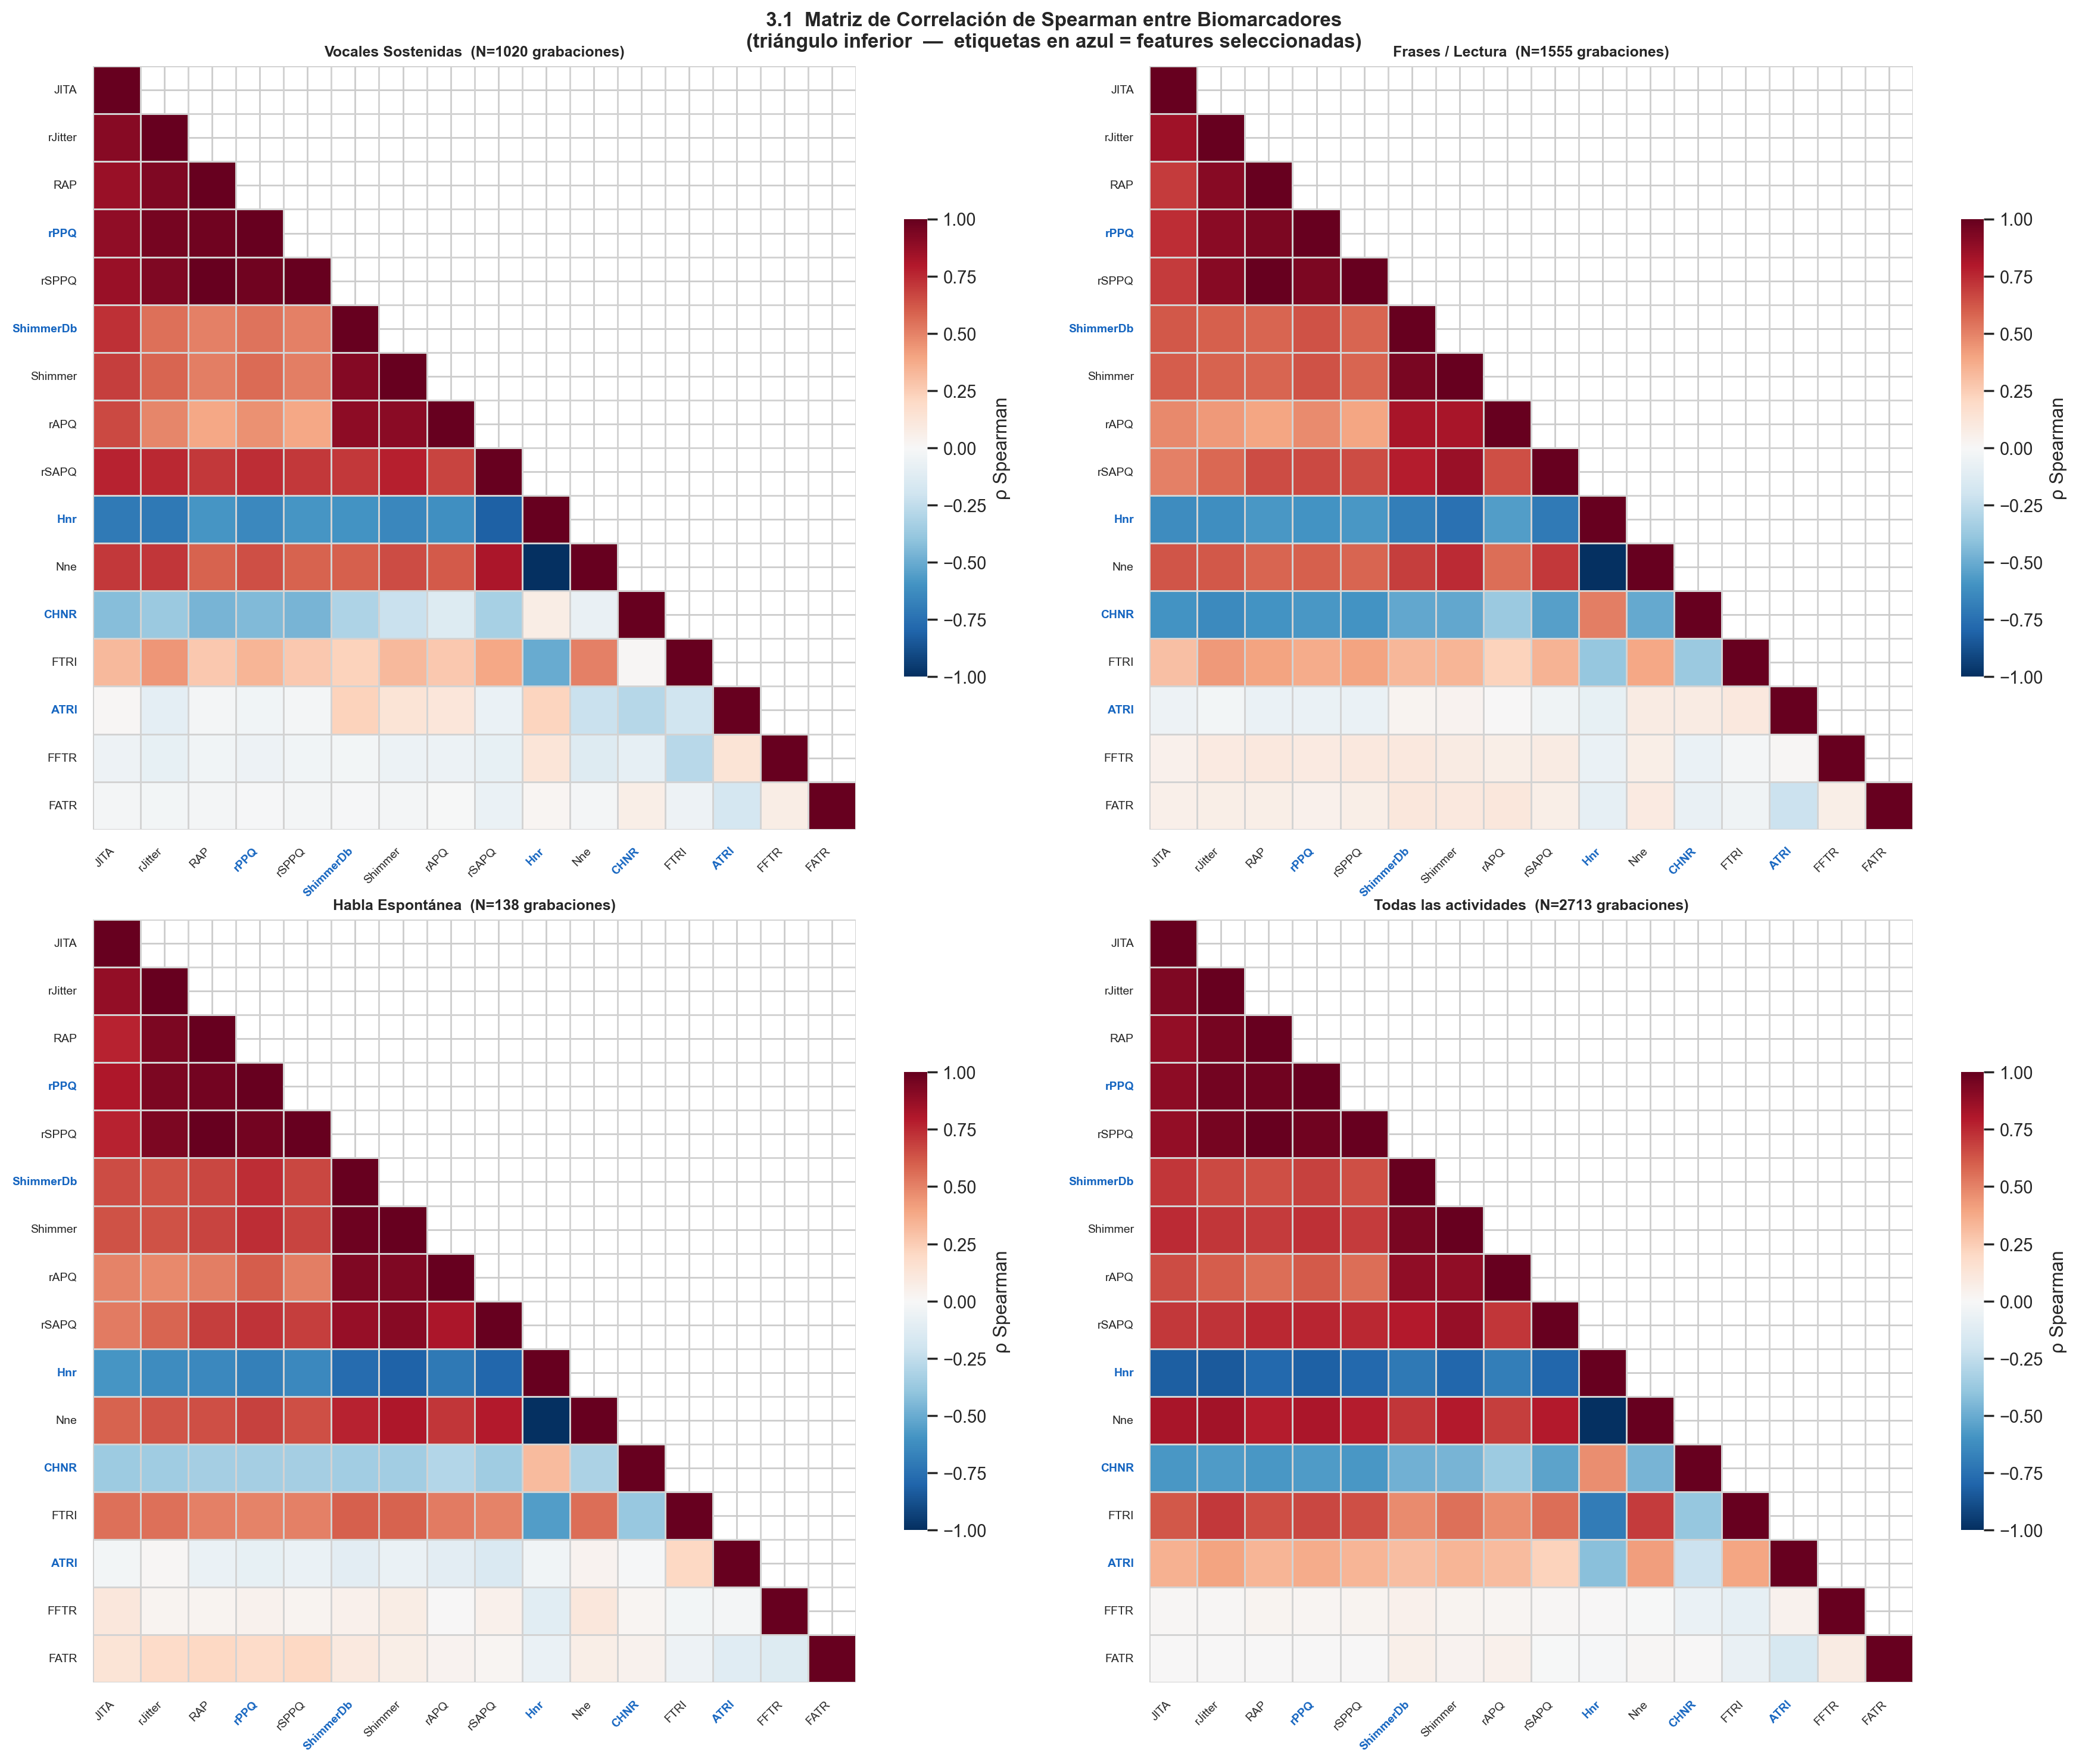
\includegraphics[width=\textwidth, height=0.34\textheight, keepaspectratio]{imagenes/eda/eda_09_corr_features.png}
                \caption{Matriz de correlación de Spearman inter-variable (triángulo inferior). Etiquetas en azul = características seleccionadas.}
                \label{fig:correlacionCcas}
            \end{subfigure}

            \vspace{0.5em}

            \begin{subfigure}[b]{\textwidth}
                \centering
                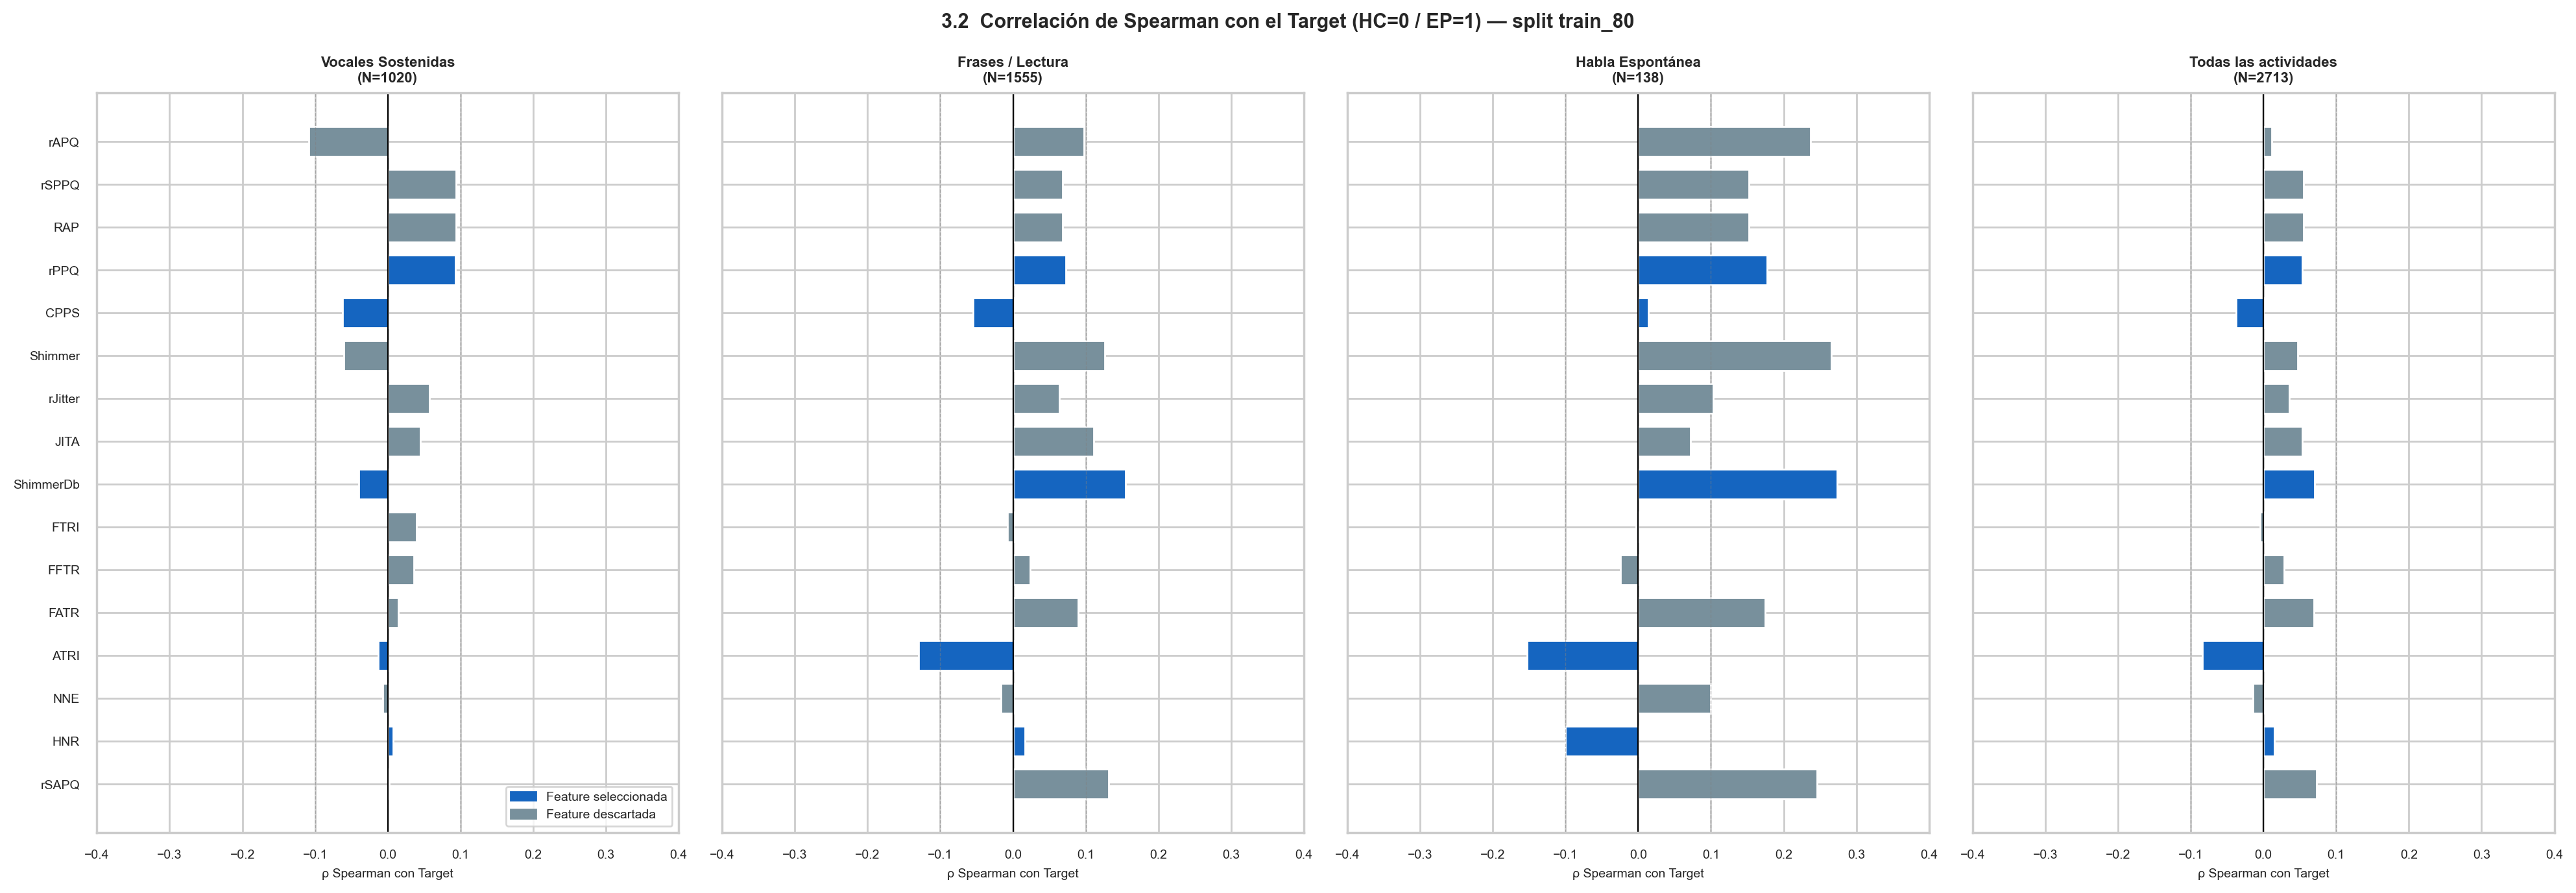
\includegraphics[width=\textwidth, height=0.21\textheight, keepaspectratio]{imagenes/eda/eda_10_corr_target.png}
                \caption{Correlación de Spearman de cada biomarcador con el \textit{Target} (HC\,=\,0 / EP\,=\,1), ordenada por valor absoluto ascendente.}
                \label{fig:correlacionClases}
            \end{subfigure}

            \vspace{0.5em}

            \begin{subfigure}[b]{\textwidth}
                \centering
                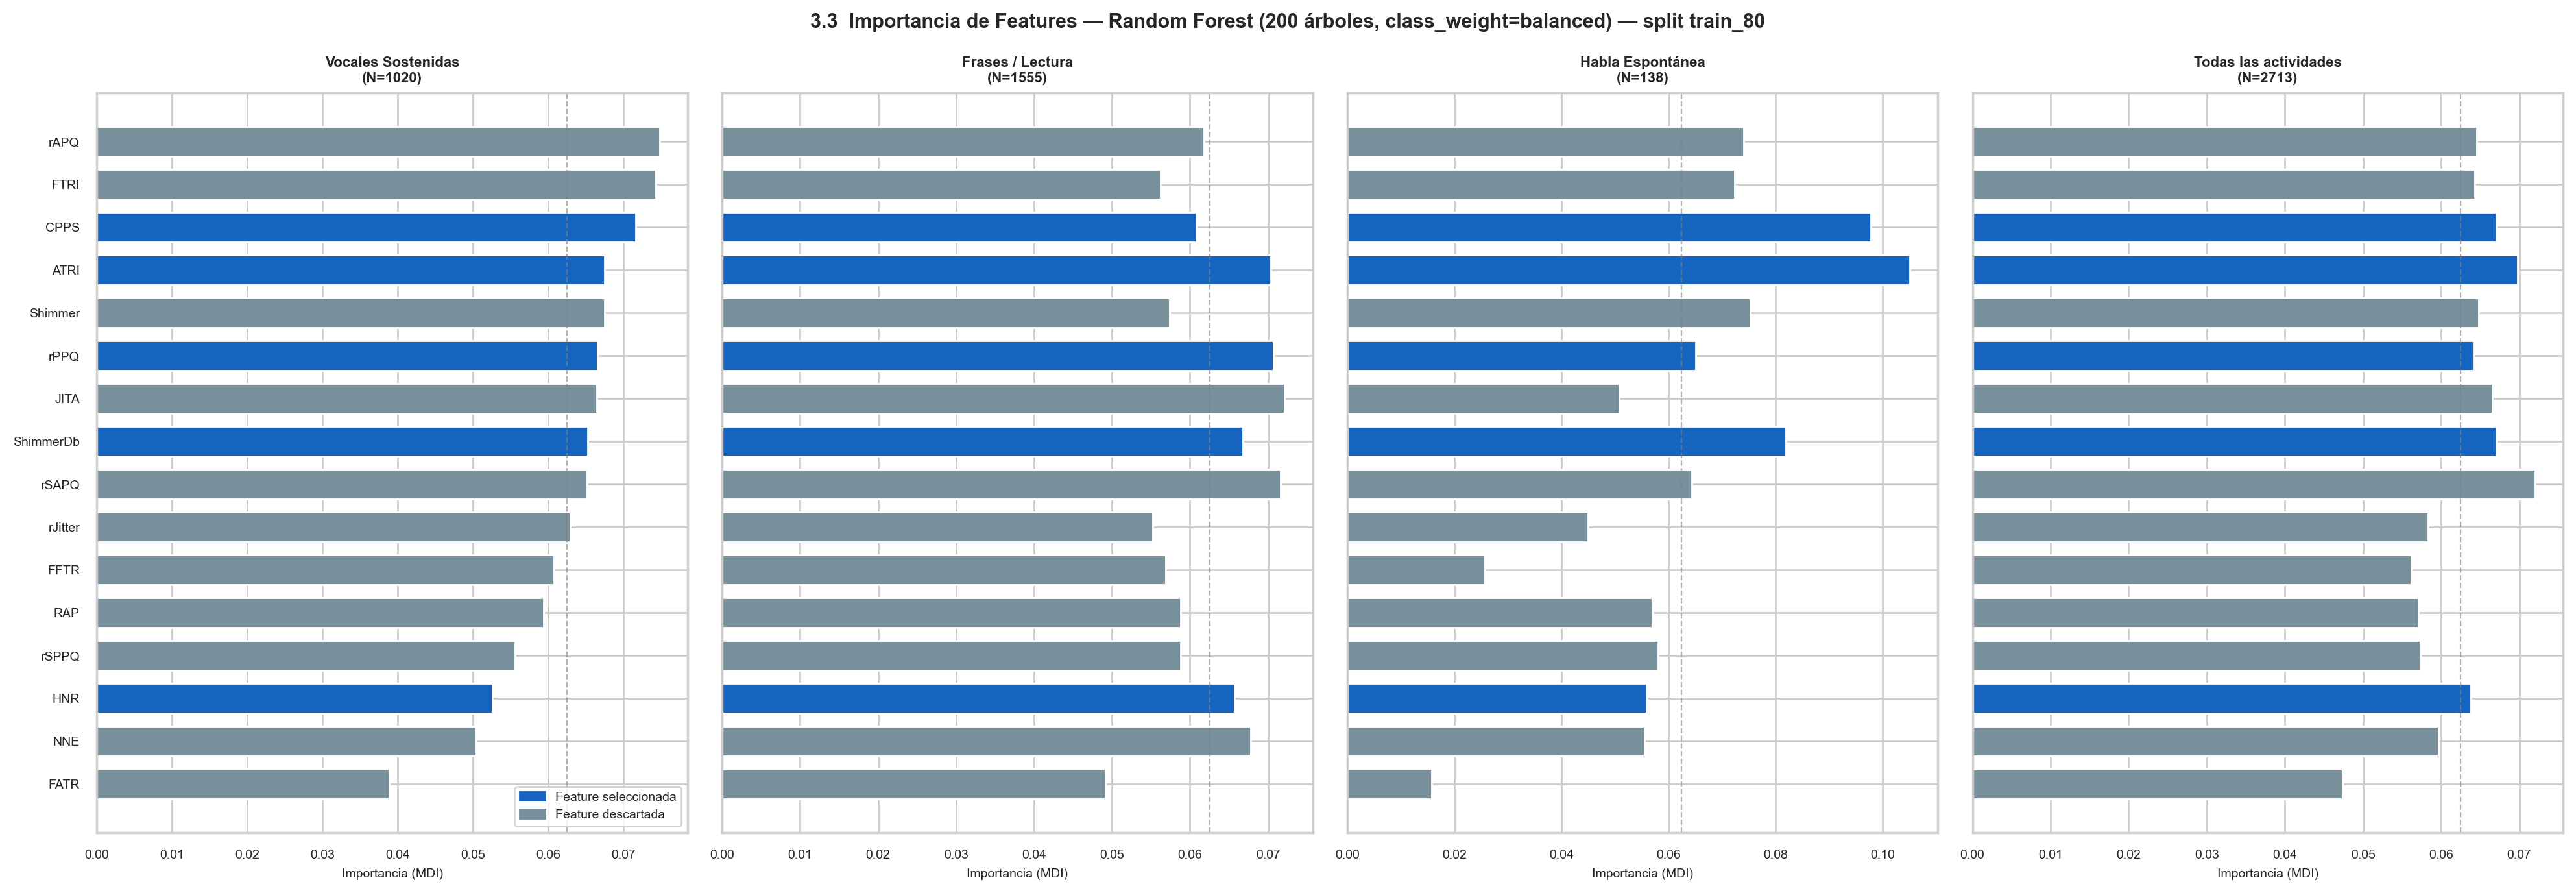
\includegraphics[width=\textwidth, height=0.21\textheight, keepaspectratio]{imagenes/eda/eda_11_rf_importance.png}
                \caption{Importancia predictiva por \textit{Random Forest} (criterio Gini). La línea discontinua marca la importancia uniforme (1/16).}
                \label{fig:pesosRF}
            \end{subfigure}

            \caption{Análisis estadísticos para la selección de características, calculados sobre el \textit{split} de entrenamiento (165 pacientes) y desglosados por actividad de habla: (a)~correlación inter-variable, (b)~correlación univariante con la clase objetivo y (c)~importancia predictiva mediante \textit{Random Forest}. Las barras y etiquetas en azul corresponden a las cinco características finalmente seleccionadas.}
            \label{fig:analisis_seleccion}
        \end{figure}


        \subsection{Análisis Estadístico de los Biomarcadores Acústicos}\label{sec:eda_features}

        Una vez completado el proceso de selección de características, se procedió a realizar un análisis estadístico descriptivo para evaluar la capacidad discriminativa preliminar de las variables seleccionadas. 

        En la Tabla~\ref{tab:medias_acusticas} se presentan las medidas de tendencia central y dispersión (media y desviación típica) de las cinco métricas fundamentales para el conjunto total de grabaciones, segmentadas por grupo diagnóstico.

        \begin{table}[H]
            \centering
            \renewcommand{\arraystretch}{1.3}
            \begin{tabularx}{0.8\textwidth}{>{\raggedright\arraybackslash}X c c}
                \toprule
                \textbf{Biomarcador Acústico} & \textbf{Control Sano (HC)} & \textbf{Parkinson (EP)} \\
                \midrule
                \textbf{rPPQ} & $0.68 \pm 0.43$ & $0.79 \pm 0.70$ \\
                \textbf{ShimmerDb} & $1.08 \pm 0.28$ & $1.12 \pm 0.31$ \\
                \textbf{HNR} & $15.88 \pm 5.42$ & $16.09 \pm 5.88$ \\
                \textbf{CPPS} & $9.79 \pm 2.05$ & $9.62 \pm 2.03$ \\
                \textbf{ATRI} & $10.89 \pm 4.91$ & $9.89 \pm 4.51$ \\
                \bottomrule
            \end{tabularx}
            \caption{Estadística descriptiva (Media $\pm$ Desviación Típica) de las características acústicas seleccionadas para sujetos de Control (HC) y pacientes con Parkinson (EP).}
            \label{tab:medias_acusticas}
        \end{table}

        A nivel clínico, se observa empíricamente un incremento en las medidas de inestabilidad vocal (rPPQ y ShimmerDb) en el grupo patológico, congruente con la pérdida de control neuromotor característica de la disartria hipocinética. Asimismo, el índice de temblor de amplitud (ATRI) muestra una alteración en su distribución. 

        El análisis estadístico exhaustivo de la totalidad de las variables extraídas inicialmente, así como las representaciones gráficas de sus distribuciones, diagramas de violín y matrices de dispersión, se encuentran detallados de forma íntegra en el \textbf{\hyperref[app:eda]{Apéndice C}}.


            

        \subsection{Generación de representaciones acústicas para Deep Learning}
        \label{sec:espectrogramas}

        A diferencia de los algoritmos de aprendizaje automático clásico, las arquitecturas de aprendizaje profundo (Deep Learning) basadas en Redes Neuronales Convolucionales (CNN) destacan por su capacidad para extraer características latentes directamente desde matrices bidimensionales. Por consiguiente, se diseñó un pipeline paralelo para transformar las señales acústicas unidimensionales en representaciones de tiempo-frecuencia, específicamente \textbf{espectrogramas en escala Mel}.

        La elección de la escala Mel frente a un espectrograma lineal estándar radica en su naturaleza logarítmica, la cual emula con mayor fidelidad la resolución perceptiva del sistema auditivo humano \cite{stevens1937}. Esta compresión del espectro otorga mayor peso y resolución a las frecuencias bajas e intermedias, banda donde residen los formantes principales de la voz humana y las micro-fluctuaciones asociadas a la disartria parkinsoniana.

        El proceso de conversión acústico-visual se llevó a cabo aplicando la Transformada Corta de Fourier (STFT, por sus siglas en inglés) sobre las señales previamente preprocesadas a 16 kHz, implementando el flujo a través de la librería \textit{librosa} \cite{mcfee2015}. Los hiperparámetros matemáticos empleados para la generación computacional de los espectrogramas fueron los siguientes:

        \begin{itemize}
            \item \textbf{Tamaño de la ventana (n\_fft):} Se fijó en 512 muestras, proporcionando una resolución frecuencial adecuada para aislar perturbaciones micromotoras.
            \item \textbf{Desplazamiento temporal (hop\_length):} Se calculó dinámicamente como el 3\,\% de la frecuencia de muestreo (aproximadamente 480 muestras a 16 kHz) entre ventanas consecutivas.
            \item \textbf{Función de enventanado (\textit{Window function}):} Se aplicó la ventana estándar de Hann (por defecto en la implementación matemática de la librería) para mitigar las fugas espectrales (\textit{spectral leakage}) en los extremos de cada segmento.
            \item \textbf{Filtros Mel (n\_mels):} El banco de filtros se configuró para proyectar el espectro sobre 65 bandas Mel.
        \end{itemize}

        Posteriormente, la matriz de densidad espectral de potencia resultante ($S$) fue convertida a una escala logarítmica de decibelios (dB) siguiendo la ecuación $S_{dB} = 10 \cdot \log_{10}(S / S_{ref})$, tomando como referencia la amplitud máxima. 

        En la \autoref{fig:ejemplo_espectrograma} se ilustra una comparativa visual entre los espectrogramas extraídos para un paciente patológico y un sujeto de control.

        \begin{figure}[H]
        \centering
        % Espectrograma Sujeto Sano
        \begin{subfigure}[b]{0.48\textwidth}
            \centering
            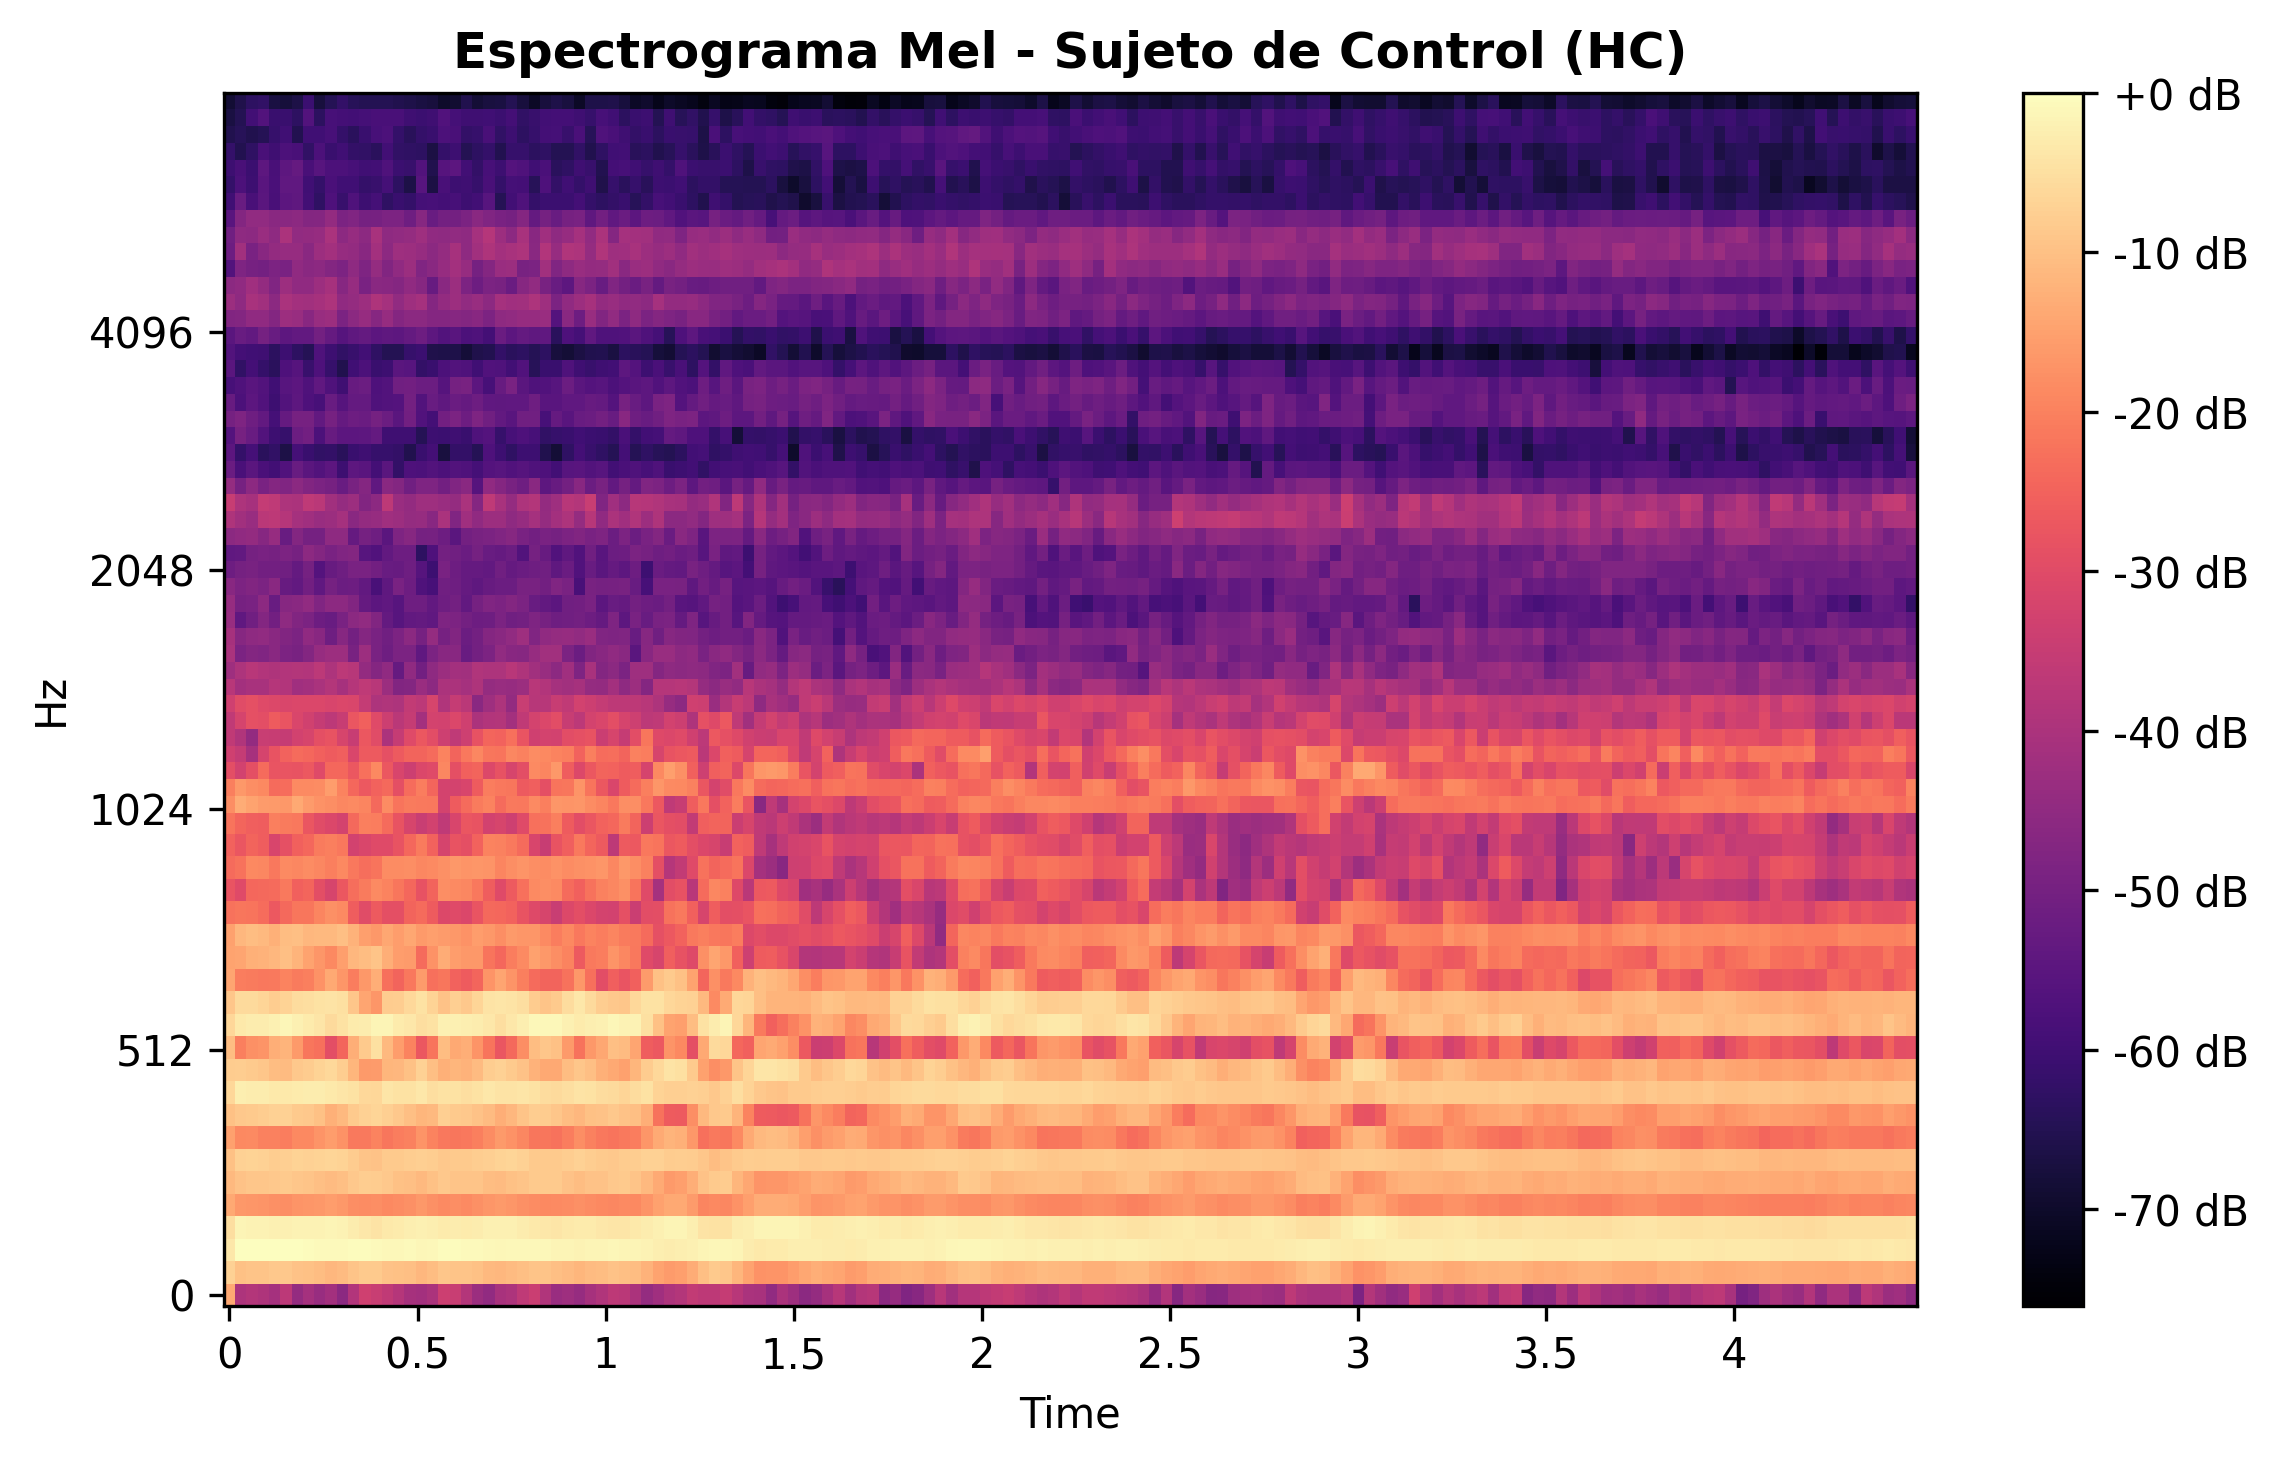
\includegraphics[width=\textwidth]{imagenes/espectrograma_sano.png}
            \caption{Sujeto de Control (HC)}
            \label{fig:spec_sano}
        \end{subfigure}
        \hfill
        % Espectrograma Paciente Parkinson
        \begin{subfigure}[b]{0.48\textwidth}
            \centering
            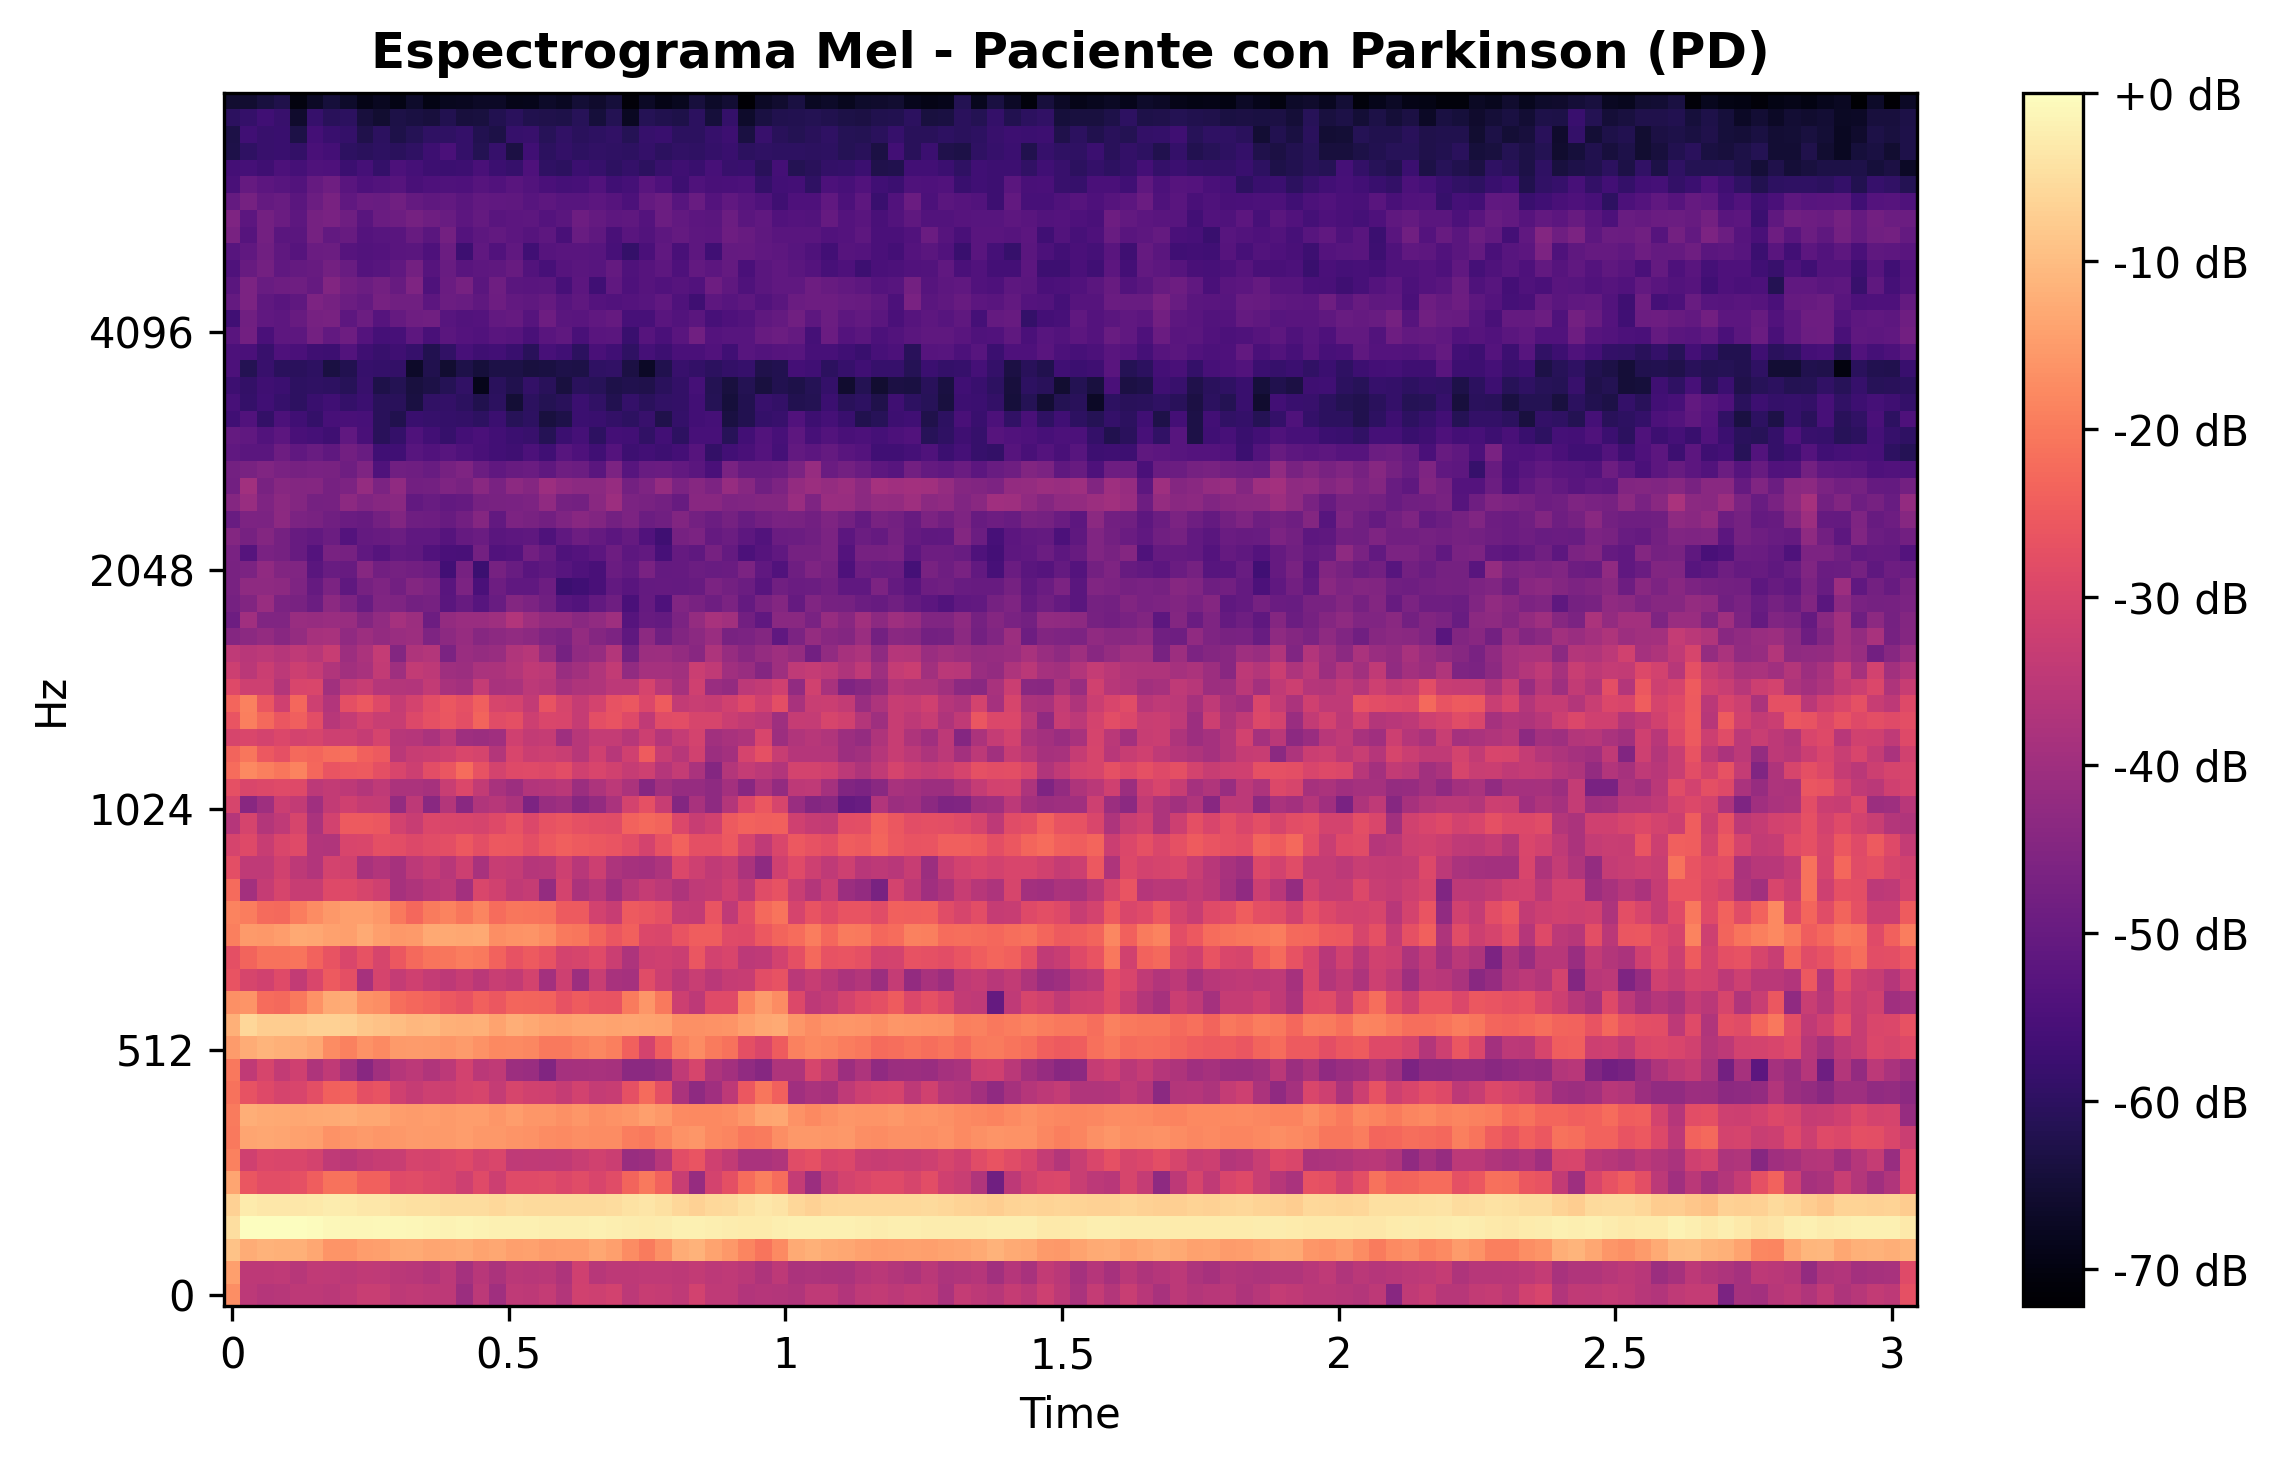
\includegraphics[width=\textwidth]{imagenes/espectrograma_parkinson.png}
            \caption{Paciente con Parkinson (PD)}
            \label{fig:spec_parkinson}
        \end{subfigure}
        
        \caption{Comparativa visual de espectrogramas en escala Mel generados con un banco de 65 filtros y una ventana de 512 muestras. Se observa la representación acústico-visual de un sujeto de control sano frente a las alteraciones y micro-fluctuaciones típicas de un paciente con Enfermedad de Parkinson.}
        \label{fig:ejemplo_espectrograma}
    \end{figure}


    \subsection{Extracción de embeddings acústicos mediante Wav2Vec 2.0}

    De forma complementaria a la extracción de características acústicas manuales y a la generación de espectrogramas, se exploró el uso de modelos fundacionales de aprendizaje profundo para la obtención de representaciones latentes de alto nivel (\textit{embeddings}). Para este propósito, se implementó la arquitectura \textbf{Wav2Vec 2.0} \cite{baevski2020}, un modelo de vanguardia desarrollado por Meta AI basado en aprendizaje auto-supervisado (\textit{Self-Supervised Learning}).

    A diferencia de las métricas clásicas, Wav2Vec 2.0 procesa la forma de onda cruda para extraer un contexto acústico denso, lo que resulta especialmente útil para capturar las sutilezas neuromotoras de la voz patológica sin necesidad de un etiquetado previo alineado fonéticamente \cite{baevski2020}. Se seleccionó específicamente la variante preentrenada \texttt{jonatasgrosman/wav2vec2-large-xlsr-53-spanish}, una adaptación del modelo XLSR-53 de Meta AI preentrenada en 53 idiomas y ajustada finamente (\textit{fine-tuned}) sobre corpus de habla espontánea en español. Esta elección responde a la naturaleza lingüística de los corpus clínicos empleados (NeuroVoz y PC-GITA, ambos en castellano), garantizando que las representaciones latentes extraídas capturen las propiedades fonéticas específicas del español sin depender de un preentrenamiento exclusivamente multilingüe.

    El pipeline de extracción automatizada se diseñó haciendo uso del ecosistema PyTorch y la librería \textit{Transformers}. El flujo de procesamiento por cada archivo de audio siguió las siguientes etapas matemáticas y computacionales:

    \begin{itemize}
        \item \textbf{Acondicionamiento de la señal:} Las muestras se cargaron a través de \textit{torchaudio}, forzando la conversión a formato mono (promediando los canales espaciales). Seguidamente, se aplicó un remuestreo dinámico a 16 kHz, requisito arquitectónico estricto impuesto por los datos de preentrenamiento del modelo Wav2Vec 2.0 \cite{wolfTransformersStateoftheArtNatural2020}.
        
        \item \textbf{Inferencia y estado latente:} La señal normalizada se introdujo en el modelo en modo de evaluación (\texttt{model.eval()}). Para garantizar la eficiencia en memoria y acelerar el cómputo en la unidad de procesamiento gráfico (GPU), el cálculo de tensores se aisló del grafo de retropropagación (\texttt{torch.no\_grad()}) \cite{paszke2019}.
        
        \item \textbf{Agrupamiento Global (\textit{Global Average Pooling}):} La arquitectura devuelve una secuencia temporal de estados ocultos correspondientes a la última capa del \textit{Transformer} (\textit{last\_hidden\_state}) \cite{wolfTransformersStateoftheArtNatural2020}. Para colapsar esta secuencia temporal (de longitud variable según la duración del audio) en un único vector de longitud fija por paciente, se aplicó la media aritmética sobre el eje temporal. 
    \end{itemize}

    El resultado de esta operación (\textit{pooling}) proyecta cada grabación de voz en un espacio vectorial continuo de \textbf{1024 dimensiones}. Este vector resultante codifica de forma abstracta las propiedades fonéticas y prosódicas del locutor, y fue exportado en formato tabular para su posterior ingestión como vector de características (\textit{feature vector}) en los modelos predictivos de Machine Learning.      
